\documentclass{article}

\usepackage[english]{babel}     
\usepackage[utf8]{inputenc}     % accent symbols
\usepackage[T1]{fontenc}
\usepackage{lmodern}
\usepackage{microtype}
\usepackage{natbib}
\usepackage{tocbibind}          
\usepackage{amsmath}            % math symbols
\usepackage{amsthm}             % math symbols
\usepackage[colorlinks=true,linkcolor=red]{hyperref} % hyper link

% for code
\usepackage{listings}
\usepackage{color,xcolor}
\definecolor{mygreen}{rgb}{0,0.6,0}
\definecolor{mygray}{rgb}{0.9,0.9,0.9}
\definecolor{mymauve}{rgb}{0.58,0,0.82}
\lstset{
backgroundcolor=\color{mygray},
numbers=left,                    
columns=fullflexible,
breaklines=true,      
captionpos=b,         
tabsize=4,            
commentstyle=\color{mygreen}, 
escapeinside={\%*}{*)},       
keywordstyle=\color{blue},    
% stringstyle=\color{mymauve}\monaco,
frame=single,                        
rulesepcolor=\color{red!20!green!20!blue!20},
% identifierstyle=\color{red},
%% language=c++,
basicstyle=\tiny
}

\usepackage{indentfirst}
\setlength{\parindent}{2em}
\usepackage[onehalfspacing]{setspace}
% graph
\usepackage{pdfpages}
\usepackage{graphicx}
% box
\usepackage{booktabs}
\usepackage{tcolorbox}

%% user defined command
\newcommand{\keyword}[1]{\textbf{#1}}
\newcommand{\keywords}[1]{\textbf{#1}}
\newcommand{\lcmd}[1]{\texttt{#1}}
\newcommand{\head}[1]{\textnormal{\textbf{#1}}}
\newcommand{\itwords}[1]{\textit{#1}}

\usepackage{float}
% all symbols
\usepackage{tipa}
\usepackage{tipx}

\usepackage{datetime}
% \usepackage{movie15}


% variable
% TODO
\newcommand{\pdfauthor}{李明明}
\newcommand{\pdftitle}{工作}
\newcommand{\pdfsubject}{工作中的经验与教训}
\newcommand{\pdfkeywords}{工作经验与教训}
\newcommand{\bookname}{工作收获}
\newcommand{\bookoneword}{工作中吸取的经验和教训}
\newcommand{\timeandcompany}{2020年12月1日}

\usepackage{bm}
\usepackage{amsfonts}

\begin{document}
\title{Coding Interview Strategy}
\maketitle{}
\newpage{}


\section{The Interview Process}

\subsection{The Basics}

\subsubsection{Do I need to know this "big O" stuff?}

Well, it depends. There are different types of interviews.

There’s the classic algorithmic coding interview, sometimes called the “Google-style whiteboard interview.” It’s focused on data structures and algorithms (queues and stacks, binary search, etc).


For startups and smaller shops, it’s a mixed bag. Most will ask at least a few algorithmic questions. But they might also include some role-specific stuff, like Java questions or SQL questions for a backend web engineer. They’ll be especially interested in your ability to ship code without much direction. You might end up doing a code test or pair-programming exercise instead of a whiteboarding session.


To make sure you study for the right stuff, you should ask your recruiter what to expect. Send an email with a question like, “Is this interview going to cover data structures and algorithms? Or will it be more focused around coding in X language.” They’ll be happy to tell you.

\subsubsection{Which programming language should I use?}

Companies usually let you choose, in which case you should use your most comfortable language. If you know a bunch of languages, prefer one that lets you express more with fewer characters and fewer lines of code, like Python or Ruby. It keeps your whiteboard cleaner.


\subsubsection{What should I wear?}

A good rule of thumb is to dress a tiny step above what people normally wear to the office.

\subsubsection{Should I send a thank-you note?}

Thank-you notes are nice, but they aren’t really expected. Be casual if you send one. No need for a hand-calligraphed note on fancy stationery. Opt for a short email to your recruiter or the hiring manager. Thank them for helping you through the process, and ask them to relay your thanks to your interviewers.


\subsection{Impostor Syndrome}

\begin{verbatim}
“It's a fluke that I got this job interview...”

“I studied for weeks, but I’m still not prepared...”

“I’m not actually good at this. They’re going to see right through me...”
\end{verbatim}

If any of these thoughts resonate with you, you're not alone. They are so common they have a name: impostor syndrome.

It’s that feeling like you’re on the verge of being exposed for what you really are—an impostor. A fraud.

\important{Impostor syndrome is like kryptonite to coding interviews.} It makes you give up and go silent.

You might stop asking clarifying questions because you’re afraid they’ll sound too basic. Or you might neglect to think out loud at the whiteboard, fearing you’ll say something wrong and sound incompetent.

You know you should speak up, but the fear of looking like an impostor makes that really, really hard.

\important{Here’s the good news: you’re not an impostor.} You just feel like an impostor because of some common cognitive biases about learning and knowledge.

Once you understand these cognitive biases—where they come from and how they work—you can slowly fix them. You can quiet your worries about being an impostor and keep those negative thoughts from affecting your interviews.


\subsubsection{Everything you could know}

Here’s how impostor syndrome works.

Software engineering is a massive field. There’s a huge universe of things you could know. Huge. Shown in Figure \ref{fig:you-could-know}.

\begin{figure}[!ht]
  \centering
  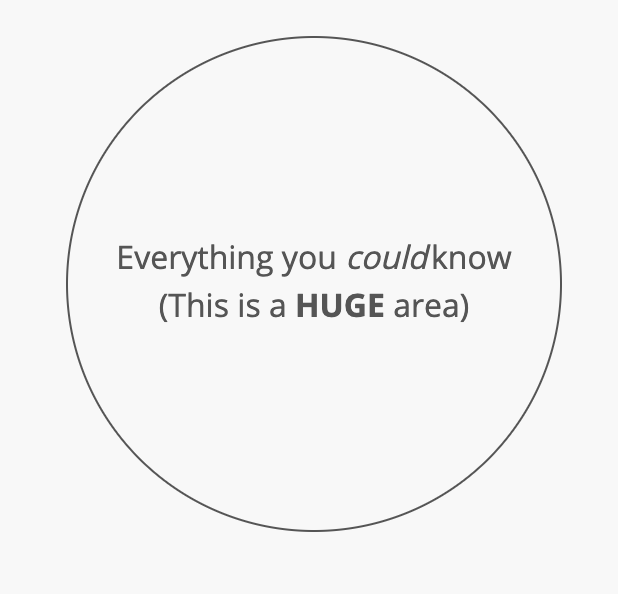
\includegraphics[width=0.5\textwidth]{pics/you-could-know}
  \caption{Everything you should know}
  \label{fig:you-could-know}
\end{figure}


In comparison to the vast world of things you could know, the stuff you actually know is just a tiny sliver. Shown in Figure \ref{fig:you-do-know}.

\begin{figure}[!ht]
  \centering
  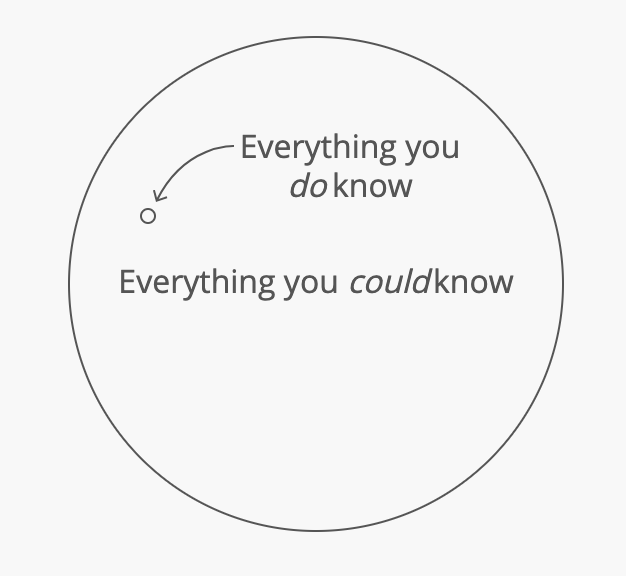
\includegraphics[width=0.5\textwidth]{pics/you-do-know}
  \caption{Everything you do know}
  \label{fig:you-do-know}
\end{figure}

 

That’s the first problem. \important{It feels like you don’t really know that much, because you only know a tiny sliver of all the stuff there is to know.}


\subsubsection{The expanding universe}

It gets worse: \important{counterintuitively, as you learn more, your sliver of knowledge feels like it's shrinking.}

That's because you brush up against more and more things you don’t know yet. Whole disciplines like machine learning, theory of computation, and embedded systems. Things you can't just pick up in an afternoon. Heavy bodies of knowledge that take months to understand.

So the universe of things you could know seems to keep expanding faster and faster—much faster than your tiny sliver of knowledge is growing. It feels like you'll never be able to keep up.


\subsubsection{What everyone else knows}

Here's another common cognitive bias: we assume that because something is easy for us, it must be easy for everyone else. So when we look at our own skills, we assume they're not unique. But when we look at other people's skills, we notice the skills they have that we don't have.

The result? We think everyone’s knowledge is a superset of our own (Figure \ref{fig:false-what-everyone-else-know}):

\begin{figure}[!ht]
  \centering
  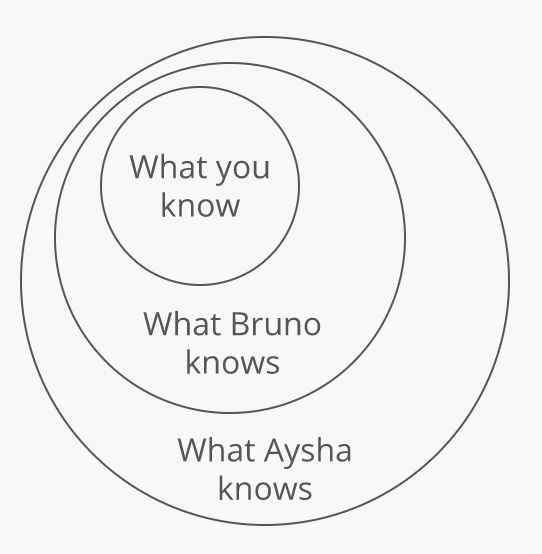
\includegraphics[width=0.5\textwidth]{pics/false-what-everyone-else-know}
  \label{fig:false-what-everyone-else-know}
\end{figure}


This makes us feel like everyone else is ahead of us. Like we're always a step behind.

But the truth is more like this (Figure \ref{fig:true-what-everyone-else-know}):

\begin{figure}[!ht]
  \centering
  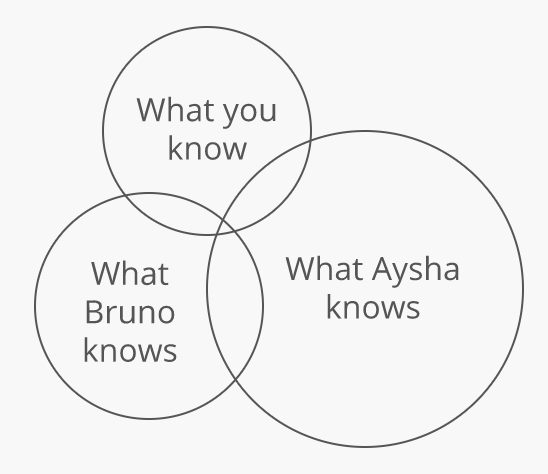
\includegraphics[width=0.5\textwidth]{pics/true-what-everyone-else-know}
  \label{fig:true-what-everyone-else-know}
\end{figure}


There's a whole area of stuff you know that neither Aysha nor Bruno knows. An area you're probably blind to, because you're so focused on the stuff you don't know.


\subsubsection{It's a problem of focus}

Focusing on what you don't know causes you to underestimate what you do know. And that's what causes impostor syndrome.

By looking at the vast (and expanding) universe of things you could know, you feel like you hardly know anything.

And by looking at what Aysha and Bruno know that you don't know, you feel like you're a step behind.

And interviews make you really focus on what you don't know. You focus on what could go wrong. The knowledge gaps your interviewers might find. The questions you might not know how to answer.

But remember:

Just because Aysha and Bruno know some things you don't know, doesn't mean you don't also know things Aysha and Bruno don't know.

And more importantly, everyone's body of knowledge is just a teeny-tiny sliver of everything they could learn. We all have gaps in our knowledge. We all have interview questions we won't be able to answer.

You're not a step behind. You just have a lot of stuff you don't know yet. Just like everyone else.



\subsection{Organizing Your Interview Timeline}

\subsubsection{Work backwards from a signing date}

\important{Pick a "signing date" and stick to it.}
This is the date that you plan to make a final decision and sign an offer. This includes some allowed time for negotiating once you have all your offers in hand (more on that later).

\subsubsection{How far out should my signing date be?}

It depends. At a high level, you should allow as much time as you can afford to. Most people underestimate how long their job search is going to take. And when you end up in a time crunch at the end, it means less time at the negotiation stage. So allowing an extra week for your job search could literally mean earning tens of thousands of dollars more in your final salary.

If you have a current job or are a full-time student, try to allow more time by starting the process earlier.

Of course, some of us will be in situations where we really need to start our new job as soon as possible. That's fine. Do what works for you.

Keep in mind that you’re shooting for having enough time to practice and get through the whole interview process with multiple companies if you can. Think through how much time you can devote to each of these steps:

\begin{itemize}
\item Studying (1–8 weeks)
\item Phone screens (1–3 weeks)
\item Onsites (1–3 weeks)
\item Negotiation (1–2 weeks)
\end{itemize}


One more consideration: if you have the means, consider leaving yourself some time for a vacation before starting your new job. Job hunting is stressful. And that window of time between signing a new offer and starting a new job can be a rare window of low stress and low responsibility in your life.



\subsubsection{Cast a wide net}

\important{Interview with multiple companies.} Exactly how many companies depends on your situation, but the point is to avoid putting all your eggs in one basket. You want multiple offers by the end, so you can negotiate the best offer possible.

A good rule of thumb: send out applications to more places than you’re currently planning. If you end up getting too many interviews…well that’s a good problem to have! You can always "pause" or simply cancel the interview process with some companies.

\important{Schedule your favorite companies last.} Get interview practice with the places you aren’t as excited about. You’ll be in your prime by the time you interview with your top choices, so long as you don’t burn out.

\important{Jot down your impressions after each interview.} You’ll be surprised how much different companies can start to melt together after a couple weeks of interviewing.


\subsubsection{Avoid burnout}

If you’re casting a wide net and allowing several weeks for your job search, you need to be careful about burnout. The interview process is a marathon, not a sprint.

\important{Space out your onsites.} Onsites are draining. Try to keep at least a two day buffer between them—one day to recover after your last onsite, and one day to get ready for the next.

\important{Don’t travel too much.} You can quickly burn yourself out bopping across the country. When you have to travel for an interview, try to wait a few days before you travel again.

Batch interviews that are in cities you have to fly to. Try to avoid flying to the same city multiple times—though sometimes traveling to the same place twice is better than trying to cram three or more onsites into a short span of time.


\subsection{Behavioral Questions}

\subsubsection{“Show, don’t tell”}

It’s good advice. When it comes to answering behavioral questions (like “Tell me about yourself”) in coding interviews, the difference between a good answer and a great answer comes down to showing rather than telling.


The problem is, people who give you the advice of “Show, don’t tell”… are themselves failing to follow it. They’re telling you to show, but they should be showing you how to show. That’s the hardest part!

So here are three specific tips for showing more and telling less.


\subsubsection{Sprinkle in specific details}

Imagine two responses to the stock interview question “Tell me about yourself.”

First:
\begin{tcolorbox}
I started programming about two years ago with some personal projects. I eventually got a job at a small tech company in my home town, and I’ve been working there about a year and a half. I like my job, but I’m looking for a new challenge, which I think your company could provide.  
\end{tcolorbox}


Then:
\begin{tcolorbox}
I got started programming because I wanted to build a social network for cats. That didn’t take off, but the prototype helped me get a job at a small tech company in my home town.

Last month, I read an awesome article on Hacker News about the social network your company is building. The scaling challenges you face seem like they’ll help me grow faster and stronger than my current role will.
\end{tcolorbox}



The second response says a lot more about the candidate.

Why? Because of the specific details. An interviewer won’t remember the tenth person to say “I’m looking for a new challenge.” They will remember the person who tried to build a social network for cats and read about their company on Hacker News.

So don’t skimp on the details. \important{Look out for opportunities to use specifics}, especially if they’re at all quirky, funny, surprising, or otherwise memorable.


\subsubsection{Tell a story from your life}

Take another common question: “Why do you want to work here?”

People tend to just cross-reference their values with those of the company or team they’re interviewing with:

\begin{tcolorbox}
I’m really interested in technical blogging and open source. So I like that your company has some open-source work and contributes back to the community.  
\end{tcolorbox}


That’s a fine response. But to really wow your interviewer, try adding a specific story around those values:

\begin{tcolorbox}
  A couple years ago, when I was still new to programming, I was working on this tricky bug. I found a post on a company blog where an engineer explained how her team solved the issue. She included a code snippet she’d open-sourced. I appreciated that she took the time to write about her team’s experience and share their solution. It helped me!

  That’s how I first started getting into open source. I really wanna work with more engineers like that—who write about their work and try to help others in the community. So I was excited to see all the stuff your team shares on your blog and on the company’s Github profile.
\end{tcolorbox}



The second response just sounds more genuine. It shows a personal connection to open source and technical blogging, instead of just telling it.

Anyone can look up a company’s core values and repeat them during an interview. It’s more meaningful to \important{tell a story from your life} that shows how those values benefited you or taught you something.



\subsubsection{Use someone else’s voice}

This one’s a neat trick. Consider one more standard behavioral question: “What’s your biggest strength?”

You might tell the interviewer:

\begin{tcolorbox}
I work well with others. Even under tough circumstances, I make sure my coworkers feel supported.  
\end{tcolorbox}


But a lightly detailed story is better suited to show this strength:

\begin{tcolorbox}
  I have a coworker, Ana, who’s been an engineer for almost a decade. We worked together on this really tough, messy project.

  Towards the end, she told me, “For such a hellish project, you really made things feel sane.” I think this is my biggest strength—I work well with others, even under tough circumstances.
\end{tcolorbox}

When you respond with a story, you can refer to what other people have said about your best qualities. In this case, a ten-year tech veteran said you made a project feel less awful. That kind of praise is a lot more credible when it comes from someone else.



\subsubsection{Practice, practice, practice}

Remember these specific tricks for showing rather than telling:

\begin{enumerate}
\item Use specific, memorable details. “Social network for cats” instead of “a personal project.”
\item Tell a story from your life. “I was trying to solve a tricky bug…” instead of “I value open source contributions.”
\item Use someone else’s voice. “’You really made things feel sane‘” instead of "I work well with others."
\end{enumerate}


Try these tactics out on the questions below. Keep in mind, sometimes it’s easiest to start with a “tell” response, then spruce it up to “show.”


\begin{itemize}
\item Tell me your biggest weakness as an engineer.
\item Describe a tricky bug you’ve encountered.
\item What’s the biggest project you’ve shipped?
\item What’s your favorite programming language? Why?
\item How do you overcome interpersonal conflicts with coworkers?
\end{itemize}

\section{The heard battle: technical whiteboard interviews}


\subsection{General Strategy}

\subsubsection{Chitchat like a pro}

Before diving into code, most interviewers like to chitchat about your background. They're looking for:

\begin{description}
\item[Metacognition about coding.] Do you think about how to code well?
\item[Ownership/leadership.] Do you see your work through to completion? Do you fix things that aren't quite right, even if you don't have to? 
\item[Communication.] Would chatting with you about a technical problem be useful or painful? 
\end{description}



You should have at least one:
\begin{itemize}
\item example of an interesting technical problem you solved
\item example of an interpersonal conflict you overcame
\item example of leadership or ownership
\item story about what you should have done differently in a past project
\item piece of trivia about your favorite language, and something you do and don't like about said language
\item question about the company's product/business
\item question about the company's engineering strategy (testing, Scrum, etc)
\end{itemize}

Nerd out about stuff. Show you're proud of what you've done, you're amped about what they're doing, and you have opinions about languages and workflows.


\subsubsection{Communication}

Once you get into the coding questions, \important{communication is key}. A candidate who needed some help along the way but communicated clearly can be even better than a candidate who breezed through the question.

Understand what kind of problem it is. There are two types of problems:

\begin{enumerate}
\item Coding. The interviewer wants to see you write clean, efficient code for a problem.
\item Chitchat. The interviewer just wants you to talk about something. These questions are often either (1) high-level system design ("How would you build a Twitter clone?") or (2) trivia ("What is hoisting in Javascript?"). Sometimes the trivia is a lead-in for a "real" question e.g., "How quickly can we sort a list of integers? Good, now suppose instead of integers we had . . ."
\end{enumerate}


If you start writing code and the interviewer just wanted a quick chitchat answer before moving on to the "real" question, they'll get frustrated. Just ask, "Should we write code for this?"

\important{Make it feel like you're on a team.} The interviewer wants to know what it feels like to work through a problem with you, so make the interview feel collaborative. Use "we" instead of "I," as in, "If we did a breadth-first search we'd get an answer in $O(n)$ time." If you get to choose between coding on paper and coding on a whiteboard, always choose the whiteboard. That way you'll be situated next to the interviewer, facing the problem (rather than across from her at a table).

\important{Think out loud}. Seriously. Say, "Let's try doing it this way—not sure yet if it'll work." If you're stuck, just say what you're thinking. Say what might work. Say what you thought could work and why it doesn't work. This also goes for trivial chitchat questions. When asked to explain Javascript closures, "It's something to do with scope and putting stuff in a function" will probably get you 90\% credit.

\important{Say you don't know.} If you're touching on a fact (e.g., language-specific trivia, a hairy bit of runtime analysis), don't try to appear to know something you don't. Instead, say "I'm not sure, but I'd guess \$thing, because...". The because can involve ruling out other options by showing they have nonsensical implications, or pulling examples from other languages or other problems.


\important{Slow the eff down.} Don't confidently blurt out an answer right away. If it's right you'll still have to explain it, and if it's wrong you'll seem reckless. You don't win anything for speed and you're more likely to annoy your interviewer by cutting her off or appearing to jump to conclusions.



\subsubsection{Get unstuck}

Sometimes you'll get stuck. Relax. It doesn't mean you've failed. Keep in mind that the interviewer usually cares more about your ability to cleverly poke the problem from a few different angles than your ability to stumble into the correct answer. \important{When hope seems lost, keep poking.}



\important{Draw pictures.} Don't waste time trying to think in your head—think on the board. Draw a couple different test inputs. Draw how you would get the desired output by hand. Then think about translating your approach into code.


\important{Solve a simpler version of the problem.} Not sure how to find the 4th largest item in the set? Think about how to find the 1st largest item and see if you can adapt that approach.


\important{Write a naive, inefficient solution and optimize it later.} Use brute force. Do whatever it takes to get some kind of answer.


\important{Think out loud more.} Say what you know. Say what you thought might work and why it won't work. You might realize it actually does work, or a modified version does. Or you might get a hint.

\important{Wait for a hint.} Don't stare at your interviewer expectantly, but do take a brief second to "think"—your interviewer might have already decided to give you a hint and is just waiting to avoid interrupting.


\important{Think about the bounds on space and runtime.} If you're not sure if you can optimize your solution, think about it out loud. 


\important{Apply a common algorithmic pattern.} There are a few patterns that come up again and again in the answers to these questions. Once you know the patterns, designing an algorithm is just a matter of trying a few of them and seeing which one sticks.




\subsubsection{Get your thoughts down}

It's easy to trip over yourself. Focus on getting your thoughts down first and worry about the details at the end.



\important{Call a helper function and keep moving.} If you can't immediately think of how to implement some part of your algorithm, big or small, just skip over it. Write a call to a reasonably-named helper function, say "this will do X" and keep going. If the helper function is trivial, you might even get away with never implementing it.


\important{Don't worry about syntax.} Just breeze through it. Revert to English if you have to. Just say you'll get back to it.


\important{Leave yourself plenty of room.} You may need to add code or notes in between lines later. Start at the top of the board and leave a blank line between each line.


\important{Save off-by-one checking for the end.} Don't worry about whether your for loop should have "<" or "<=." Write a checkmark to remind yourself to check it at the end. Just get the general algorithm down.



\important{Use descriptive variable names.} This will take time, but it will prevent you from losing track of what your code is doing. Use names\_{}to\_{}phone\_{}numbers instead of nums. Imply the type in the name. Functions returning booleans should start with "is\_{}*". Vars that hold a list should end with "s." Choose standards that make sense to you and stick with them.



\subsubsection{Clean up when you're done}

\important{Walk through your solution by hand, out loud, with an example input.} Actually write down what values the variables hold as the program is running—you don't win any brownie points for doing it in your head. This'll help you find bugs and clear up confusion your interviewer might have about what you're doing.

\important{Look for off-by-one errors.} Should your for loop use a "<=" instead of a "<"?

\important{Test edge cases.} These might include empty sets, single-item sets, or negative numbers. Bonus: mention unit tests!

\important{Don't be boring.} Some interviewers won't care about these cleanup steps. If you're unsure, say something like, "Then I'd usually check the code against some edge cases—should we do that next?"



\subsection{Tricks for Getting Unstuck}

\subsubsection{When you’re stuck on getting started}

1) \important{Write a sample input on the whiteboard and turn it into the correct output "by hand."} Notice the process you use. Look for patterns, and think about how to implement your process in code.

2) \important{Solve a simpler version of the problem.} Remove or simplify one of the requirements of the problem. Once you have a solution, see if you can adapt that approach for the original question.

3) \important{Start with an inefficient solution.} Even if it feels stupidly inefficient, it’s often helpful to start with something that’ll return the right answer. From there, you just have to optimize your solution. Explain to your interviewer that this is only your first idea, and that you suspect there are faster solutions.






\subsubsection{When you’re stuck on finding optimizations}

1) \important{Look for repeat work.} If your current solution goes through the same data multiple times, you’re doing unnecessary repeat work. See if you can save time by looking through the data just once.

Say that inside one of your loops, there’s a brute-force operation to find an element in an array. You’re repeatedly looking through items that you don’t have to. Instead, you could convert the array to a lookup table to dramatically improve your runtime.

2) \important{Look for hints in the specifics of the problem.} Is the input array sorted? Is the binary tree balanced? Details like this can carry huge hints about the solution. If it didn’t matter, your interviewer wouldn’t have brought it up. It’s a strong sign that the best solution to the problem exploits it.

Suppose you’re asked to find the first occurrence of a number in a sorted array. The fact that the array is sorted is a strong hint—take advantage of that fact by using a binary search.

3) \important{Throw some data structures at the problem.} Can you save time by using the fast lookups of a hash table? Can you express the relationships between data points as a graph? Look at the requirements of the problem and ask yourself if there’s a data structure that has those properties.


4) Establish bounds on space and runtime. Think out loud about the parameters of the problem. Try to get a sense for how fast your algorithm could possibly be:


\subsubsection{When All Else Fails}


1) Make it clear where you are. State what you know, what you’re trying to do, and highlight the gap between the two. The clearer you are in expressing exactly where you’re stuck, the easier it is for your interviewer to help you.

2) Pay attention to your interviewer. If she asks a question about something you just said, there’s probably a hint buried in there. Don’t worry about losing your train of thought—drop what you’re doing and dig into her question.


\subsubsection{Relax. You’re supposed to get stuck}

Interviewers choose hard problems on purpose. They want to see how you poke at a problem you don’t immediately know how to solve.

Seriously. If you don’t get stuck and just breeze through the problem, your interviewer’s evaluation might just say “Didn’t get a good read on candidate’s problem-solving process—maybe she’d already seen this interview question before?”

On the other hand, if you do get stuck, use one of these tricks to get unstuck, and communicate clearly with your interviewer throughout...that’s how you get an evaluation like, “Great problem-solving skills. Hire.”






\subsection{Dealing With Dead Ends}

\subsubsection{Listening vs. holding your train of thought}

Finally! After a while of shooting in the dark and frantically fiddling with sample inputs on the whiteboard, you've came up with an algorithm for solving the coding question your interviewer gave you.

Whew. Such a relief to have a clear path forward. To not be flailing anymore.

Now you're cruising, getting ready to code up your solution.

When suddenly, your interviewer throws you a curve ball.

"What if we thought of the problem this way?"

You feel a tension we've all felt during the coding interview:

\important{"Try to listen to what they're saying...but don't lose your train of thought...ugh, I can't do both!"}

This is a make-or-break moment in the coding interview. And so many people get it wrong.

Most candidates end up only half understanding what their interviewer is saying. Because they're only half listening. Because they're desperately clinging to their train of thought.

And it's easy to see why. For many of us, completely losing track of what we're doing is one of our biggest coding interview fears. So we devote half of our mental energy to clinging to our train of thought.

To understand why that's so wrong, we need to understand the difference between what we see during the coding interview and what our interviewer sees.


\subsubsection{The programming interview maze}

Working on a coding interview question is like walking through a giant maze.

You don't know anything about the shape of the maze until you start wandering around it. You might know vaguely where the solution is, but you don't know how to get there. 

\begin{figure}[H]
  \centering
  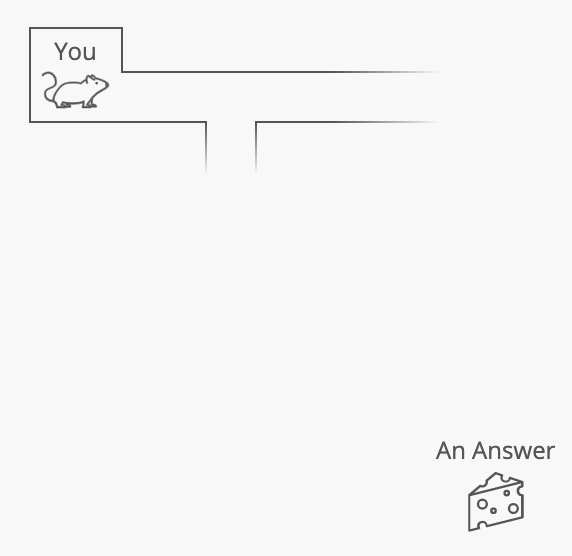
\includegraphics[width=0.5\textwidth]{pics/maze1}
  \label{fig:maze1}
\end{figure}



As you wander through the maze, you might find a promising path (an approach, a way to break down the problem). You might follow that path for a bit. 


\begin{figure}[H]
  \centering
  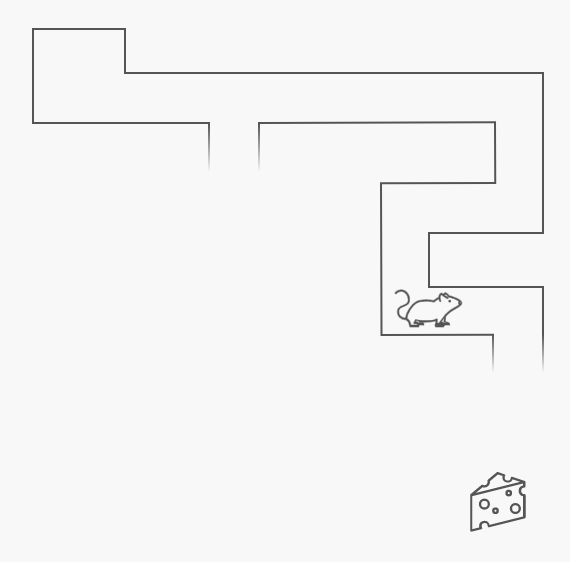
\includegraphics[width=0.5\textwidth]{pics/maze2}
  \label{fig:maze2}
\end{figure}




Suddenly, your interviewer suggests a different path: 


\begin{figure}[H]
  \centering
  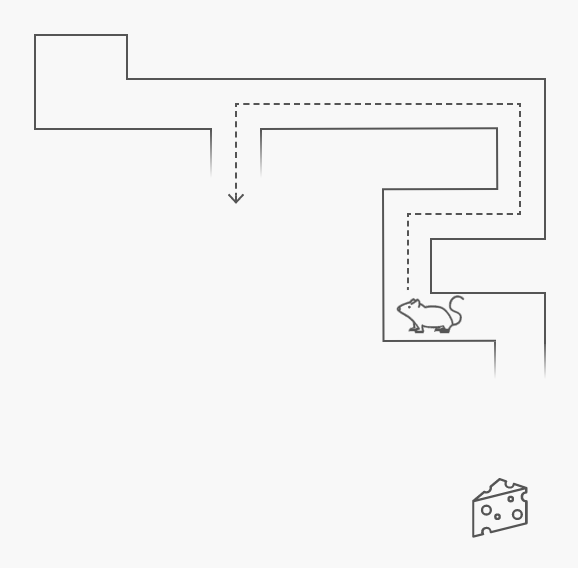
\includegraphics[width=0.5\textwidth]{pics/maze3}
  \label{fig:maze3}
\end{figure}


But from what you can see so far of the maze, your approach has already gotten you halfway there! Losing your place on your current path would mean a huge step backwards. Or so it seems.

That's why people hold onto their train of thought instead of listening to their interviewer. Because from what they can see, it looks like they're getting somewhere!

But here's the thing: \important{your interviewer knows the whole maze.} They've asked this question 100 times.


So if your interviewer is suggesting a certain path, you can bet it leads to an answer. 

\begin{figure}[H]
  \centering
  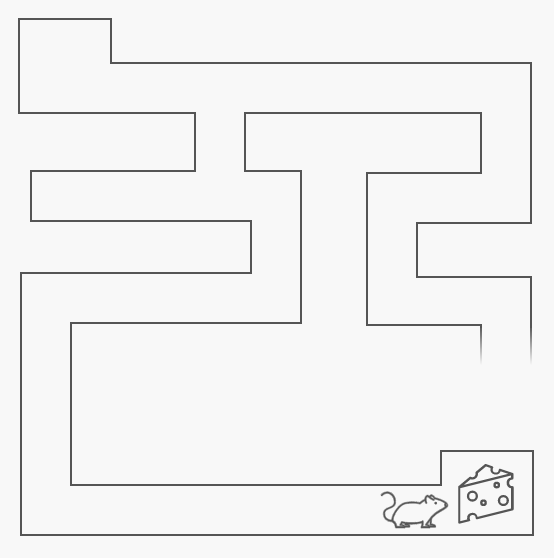
\includegraphics[width=0.5\textwidth]{pics/maze4}
  \label{fig:maze4}
\end{figure}



And your seemingly great path? There's probably a dead end just ahead that you haven't seen yet: 


\begin{figure}[H]
  \centering
  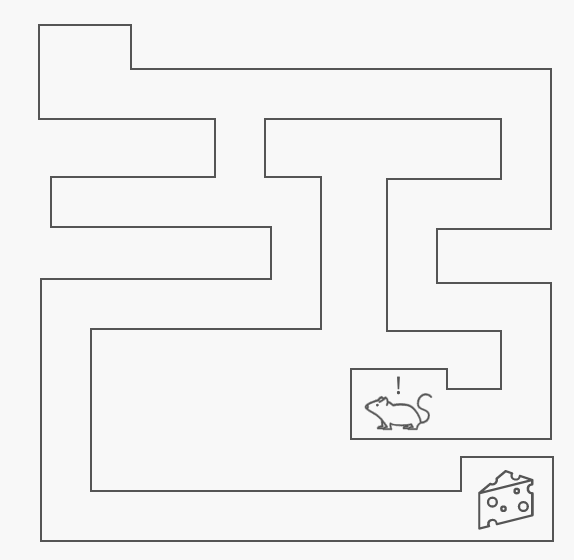
\includegraphics[width=0.5\textwidth]{pics/maze5}
  \label{fig:maze5}
\end{figure}


Or it could just be a much longer route to a solution than you think it is. That actually happens pretty often—there's an answer there, but it's more complicated than you think. 


\begin{figure}[H]
  \centering
  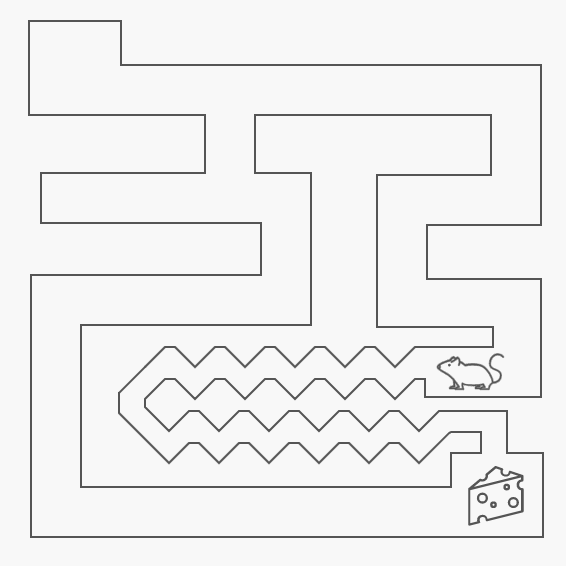
\includegraphics[width=0.5\textwidth]{pics/maze6}
  \label{fig:maze6}
\end{figure}


\subsubsection{Hitting a dead end is okay. Failing to listen is not.}

Your interviewer probably won't fault you for going down the wrong path at first. They've seen really smart engineers do the same thing. They understand it's because you only have a partial view of the maze.

They might have let you go down the wrong path for a bit to see if you could keep your thinking organized without help. But now they want to rush you through the part where you discover the dead end and double back. Not because they don't believe you can manage it yourself. But because they want to make sure you have enough time to finish the question.

But here's something they will fault you for: failing to listen to them. Nobody wants to work with an engineer who doesn't listen.

So when you find yourself in that crucial coding interview moment, when you're torn between holding your train of thought and considering the idea your interviewer is suggesting...remember this:

\important{Listening to your interviewer is the most important thing.}

Take what they're saying and run with it. Think of the next steps that follow from what they're saying.

Even if it means completely leaving behind the path you were on. Trust the route your interviewer is pointing you down.

Because they can see the whole maze.


\subsection{The 24 Hours Before Your Interview}

\important{The 24 hours before your onsite are about finding ways to maximize your performance.}
Ideally, you wanna be having one of those days, where elegant code flows effortlessly from your fingertips, and bugs dare not speak your name for fear you'll squash them.

\important{You need to get your mind and body in The Zone.}

\subsubsection{Don't study all night -- sleep!}

\important{Interviewing sleep deprived could be worse than getting drunk beforehand.}
Make it your mission to get a full night sleep, because you want all the brain power you can get.


In fact, try to get two nights of good sleep before interviewing, since sleep debt lasts a few days.


\important{As soon as the sun goes down, put down the practice problems and focus on relaxing.} If sleeping isn't your strongest skill, try these sleepytime guidelines:

\begin{itemize}
\item Exercise lightly earlier in the day.
\item Don't drink caffeine in the afternoon, and don't drink alcohol at all.
\item Avoid bright screens in the evening. Dim your screen once the sun sets.
\item Eat a light dinner, ideally one with noggin-friendly foods, like salmon, beans, and vegetables.
\item Before bed, turn on a boring podcast, listen to some calming music, or read a book.


\end{itemize}


\important{The most important thing is to not stay up late practicing new or difficult problems.} That'll only put your brain on a train to Los Anxiousness.
Instead, you should ...

\subsubsection{Practice stuff you rock at}.

\important{To cultivate your confidence, practice questions that you can already solve handily.} Sure, feel free to start the day with a new problem, but by the afternoon you should be building momentum with the questions you know best.

Giving yourself a few wins like this helps your brain simulate a stellar session at the whiteboard. You'll go to sleep dreaming of data structures, and you'll wake up with a self-esteem stimulus that makes you stand out in your interview.


\subsubsection{Imagine your best day}

\important{Write out the ideal version of your day.} It's a positive visualization exercise. This might sound like some hippie shit, but it's something athletes and entrepreneurs do all the time.

The fun part is that there isn't a ‘correct’ way to do this. It's up to you! If you're not sure where to start, here's some inspiration:
\begin{description}
\item[Greet your interviewer(s).] Play through some small talk. Maybe you make a little joke they find funny.
\item[Crush your first question.] The first question comes your way, and you write out the answer deftly. Your interviewer's face looks impressed.
\item[Overcome a tough question.] You get a trickier part of a problem. You feel some adrenaline, but you keep calm. You ask a few clarifying questions and carry on to a solution.
\item[End the day on a high note.] Your last interview of the day involes talking to a director or VP, and the conversation is lively. You leave the building smiling and feeling great about the whole experience.
\end{description}


\important{Visualiing a successful day will build your confidence.} You're training your brain to expect success and feel more comfortable during your interview.



\subsubsection{Walk through your problem solving process}

\important{Reinforcing problem-solving patterns goes a longer way than practicing new problems} in the hours leading up to your interview. 

\begin{enumerate}
\item Brainstorm an algorithm. Draw out sample inputs and play around with them while talking and thinking out loud. Don't start writing code until you and your interviewer feel good about your algorithm.
\item Barf out your algorithm in code. Focus on getting it all down first, and jot down notes next to the things you wanna go back and double-check later.
\item Debug your code. Walk through your code with sample input, look for off-by-one-errors and other bugs.
\end{enumerate}



This high-level, “What's my problem solving process” is great to keep thinking about the morning of your interview. And speaking of that morning…




\subsubsection{Precompute your morning}
Decision fatigue is real. It's why successful people like Mark Zuckerberg and Barack Obama always wear the same thing—to minimize the number of decisions they make each morning. Luckily, it's easy to avoid decision fatigue once you're aware of it!

\important{Plan the boring stuff ahead of time.} Here are a few suggestions to get you started:

\begin{description}

\item[Pack your bag.] Include a snack and water bottle.
\item[Lay out some nice clothes.] Dress a tiny step above what others in the office are wearing (usually they'll be sporting jeans and a t-shirt).
\item[Plan your breakfast.] For your brain's sake, try to include eggs, berries, and avocado.
\item[Choose your route to the office.] Expect traffic. Scope out the parking situation if you're driving.
\item[Tarantino your morning.] Work backwards from about 30 minutes before your interview, and figure out what time you need to wake up.
\item[Set an alarm (or ten).] Remember that you want time in the morning to chill, eat a leisurely breakfast, and sip on a cup of coffee (if that's your cup of… tea).
\item[Brainstorm a pump-up routine.] Come up with a few things to get you stoked. If you're not sure what your morning pump-up routine looks like, we've got you covered…
\end{description}


\subsubsection{Get pumped}

The morning of your interview, you wanna get energized! The right pump-up routine should make you excited, confident, and ready to tackle your interview head-on.

\important{Get your body moving.} Do sun salutations and a few jumping jacks. Light exercise increases the blood flow to your brain and helps clear your mind.

\important{Power pose and read your positive visualization.} It might feel strange at first, but it works! You'll prime yourself to feel more confident heading into your interview.

Listen to pump-up music. 



\subsection{Maximizing Your Practice}

When you start practicing for coding interviews, there’s a lot to cover. You’ll naturally wanna brush up on technical questions. But how you practice those questions will make a big difference in how well you’re prepared.

Here’re a few tips to make sure you get the most out of your practice sessions.


\subsubsection{Track your weak spots}

One of the hardest parts of practicing is knowing what to practice. Tracking what you struggle with helps answer that question.

So grab a fresh notebook. After each question, look back and ask yourself, “What did I get wrong about this problem at first?” Take the time to write down one or two things you got stuck on, and what helped you figure them out. Compare these notes to our tips for getting unstuck.

After each full practice session, read through your entire running list. Read it at the beginning of each practice session too. This’ll add a nice layer of rigor to your practice, so you’re really internalizing the lessons you’re learning.

\subsubsection{Use an actual whiteboard}

Coding on a whiteboard is awkward at first. You have to write out every single character, and you can’t easily insert or delete blocks of code.

Use your practice sessions to iron out that awkwardness. Run a few problems on a piece of paper or, if you can, a real whiteboard. A few helpful tips for handwriting code:

\begin{description}
\item[Start in the top-left corner.] You want all the room you can get.
\item[Leave blank space between each line of code.] This makes it much easier to add things later.
\item[Slow down.] Take an extra second to think of descriptive variable names. You might be tempted to move faster by using short variable names, but that actually ends up costing more time. It’ll make your code harder to debug!
\end{description}



\subsubsection{Set a timer}

Get a feel for the time pressure of an actual interview. You should be able to finish a problem in 30–45 minutes, including debugging your code at the end.

If you’re just starting out and the timer adds too much stress, put this technique on the shelf. Add it in later as you start to get more comfortable with solving problems.



\subsubsection{Think out loud}

Like writing code on a whiteboard, this is an acquired skill. It feels awkward at first. But your interviewer will expect you to think out loud during the interview, so you gotta power through that awkwardness.

A good trick to get used to talking out loud: \important{Grab a buddy}. Another engineer would be great, but you can also do this with a non-technical friend.

Have your buddy sit in while you talk through a problem. Better yet—try loading up one of our questions on an iPad and giving that to your buddy to use as a script!


\subsubsection{Set aside a specific time of day to practice.}

Give yourself an hour each day to practice. Commit to practicing around the same time, like after you eat dinner. This helps you form a stickier habit of practicing.

Prefer small, daily doses of practice to doing big cram sessions every once in a while. Distributing your practice sessions helps you learn more with less time and effort in the long run.




\end{document}

